\documentclass[12pt]{article}

\usepackage{url}
\usepackage{fullpage}
\usepackage{amssymb,amsfonts}
\usepackage{amsmath}
\newcommand{\eps}{\varepsilon}
\newcommand{\R}{\mathbb{R}}

\usepackage{listings}
\usepackage{color}
\usepackage{graphicx}
\usepackage{float}

\usepackage{tikz}
\usetikzlibrary{arrows.meta,calc,positioning}

\usepackage{varwidth}

\usepackage{amsthm}
\theoremstyle{definition}
\newtheorem{definition}{Definition}[section]

\usepackage{hyperref}
\hypersetup{
    linktoc=all,     %set to all if you want both sections and subsections linked
    colorlinks=true,
    linkcolor=blue,
    filecolor=magenta,      
    urlcolor=blue,
    citecolor=blue
}

\definecolor{dkgreen}{rgb}{0,0.6,0}
\definecolor{gray}{rgb}{0.5,0.5,0.5}
\definecolor{mauve}{rgb}{0.58,0,0.82}

\lstset{frame=tb,
  language=Python,
  aboveskip=3mm,
  belowskip=3mm,
  showstringspaces=false,
  columns=flexible,
  basicstyle={\small\ttfamily},
  numbers=none,
  numberstyle=\tiny\color{gray},
  keywordstyle=\color{blue},
  commentstyle=\color{dkgreen},
  stringstyle=\color{mauve},
  breaklines=true,
  breakatwhitespace=true,
  tabsize=3
}

\usepackage[toc,page]{appendix}

\DeclareMathOperator*{\E}{\mathbb{E}}
\let\Pr\relax
\DeclareMathOperator*{\Pr}{\mathbb{P}}

\DeclareMathOperator*{\Lap}{\text{Lap}}

\DeclareMathOperator*{\Geo}{\text{Geo}}

\def\cl{\lstinline}

\title{CS 208 Final Project:\\ A Modular System for Local Differential Privacy}
\author{Andrew Shackelford and Peter Chang}
\date{May 17, 2019}
\setcounter{tocdepth}{1}

\begin{document}

\maketitle

{
  \hypersetup{linkcolor=black, hidelinks}
  \tableofcontents
}

\newpage

\section{Research Questions}

\noindent

With this project, we aim to address several research questions.

\begin{itemize}
    \item What is the best way to implement local differential privacy?
    \item Why have large tech companies only implemented local differential privacy in small instances?
    \item What needs must a local differential privacy framework address?
    \item How could already existing local differential privacy frameworks be improved so that they are easier to implement?
\end{itemize}

Local differential privacy has been touted by many tech companies as a way to truly revolutionize collecting telemetry data. Despite these claims however, the current implementations of local differential privacy are few and far between. Apple \cite{apple} uses local differential privacy to detect new emojis, phrases, and some other small telemetry data. However, Tang et al. \cite{tang_et_al} found concerning amounts of privacy loss over multiple analytics reports. Google \cite{google} uses RAPPOR to collect analytics data from Chrome, yet has not updated the software since 2016, and is currently phasing it out. Lastly, Microsoft Research \cite{microsoft} published a paper and wrote a blog post about collecting telemetry data privately, but has not actually publicized the use of local differential privacy in any of its products.

\bigskip

As a result, the only open-source local DP product, RAPPOR, is now being phased out, and there are few if any open-source local differential privacy frameworks. While there have been many frameworks for centralized differential privacy, such as $\epsilon$ktelo \cite{ektelo}, Psi ($\Psi$) \cite{psi}, and PinQ \cite{pinq}, there exist no equivalent frameworks for local differential privacy.

\bigskip

Therefore, we aim to design and describe a modular, extensible framework for local differential privacy, so that any interested party can easily implement local DP and know that their data collection mechanism is private. If time allows, we hope to implement a small subset of the framework as a proof of concept, allowing for others to extend the framework to their needs. By doing so, we hope that we can increase utilization of differential privacy throughout the industry, and further protect the privacy of users.

\section{Past Work}

\subsection{Background}

\noindent

A \textit{centralized} model of differential privacy assumes the existence of a
trusted database administrator with direct access to private data. However,
this may be problematic for a number of reasons: a trusted administrator may be
hard to find and an aggregate database of private information raises the
possibility that an untrusted adversary may gain access to it at some future
time. \cite{dwork}

\bigskip

Therefore, the local model of differential privacy was introduced to avoid the
problem of having a database of private information at all: now each user
randomizes their own data before sending it to an aggregator. It formalizes
\textit{local differential privacy} as follows:

\begin{definition}
  A randomized algorithm $\mathcal{Q}$ is $\epsilon$-local differentially
  private if for all pairs of user's possible private data $x$, $x'$, and all
  adversarial strategies $A$, 
  \begin{align*} 
    \Pr[A(\mathcal{Q}_i(x)) = \mbox{YES}] \leq e^{\epsilon} \cdot \Pr[A(
    \mathcal{Q}_i(x')) = \mbox{YES}]
  \end{align*}
\end{definition}

There exist many local differentially private algorithms $\mathcal{Q}$, such as \textit{Randomized Response}, \textit{Hadamard Count Mean Sketch}, and \textit{Sequence Fragment Puzzle}, among many others.

\subsection{Google}

\noindent

Google developed and deployed Randomized Aggregatable Privacy-Preserving Ordinal Response (RAPPOR) to collect statistics through Google's Chrome Web browser.

\bigskip

RAPPOR employs two stages of randomized response. First, using a Bloom filter containing the client's private data, it generates a ``fake Bloom filter" whose bits are determined via randomized response using the original Bloom filter's bits. This filter is memoized and permanently reused when reporting the client's particular value it represents. Next, a bit array is generated with its bit elements determined via randomized response using the bits of the fake Bloom filter from the previous step. This randomization step is recomputed for each transmission of data.

\bigskip

Note that since the first randomization step is not reversible via averaging over repeated observations, it ensures long-term privacy. On the other hand, the second randomization step, which is reversible via averaging, makes it very difficult for adversaries to uniquely identify a client based on the values of the permanent Bloom filter, and hence ensures short-term privacy.

\subsection{Apple}

\noindent

Apple uses local differential privacy in several use cases in order to learn more about its users' habits, specifically estimating the frequencies of elements, without compromising privacy. Its main use cases include determining which emojis are popular, identifying websites that high resource usage or crash often, or determining which custom phrases are popular.

\bigskip

In contrast to Google, Apple does not employ two stages of randomized response. Instead, Apple immediately discards any identifying information, including IP address, as soon as the information is received at the server. Only then is the data ingested, aggregated, and eventually analyzed.

\bigskip

In order to reduce transmission costs, Apple utilizes both the Count Mean Sketch and the Hadamard Count Mean Sketch algorithms to decrease the sizes of the resulting differentially private vectors. Apple also uses the Sequence Fragment Puzzle algorithm in order to detect new phrases without having to loop through all possible combinations.

\subsection{Ektelo}

\noindent

Ektelo is a modular framework for centralized differential privacy, developed by researchers at UMass Amherst, Duke, and Colgate University. We chose to look at Ektelo and other differential privacy frameworks so that we could examine the benefits and drawbacks of current implementations. Ektelo was particularly insightful for the modularity of its framework. Ektelo compartmentalizes each of its functions based on the effects they could have on privacy, so users of the framework have to pay as little attention as possible to the privacy implications of their analysis.

\bigskip

Since Ektelo already has its differentially private functions built-in, any analyst is essentially given privacy ``for free'' since Ektelo ensures that any queries or transformations on the data are differentially private. This is another crucial component of Ektelo -- the private-public barrier that ensures that privacy is not compromised no matter what queries are performed. Lastly, Ektelo has the concept of ``plans'' -- where Ektelo uses properties of differential privacy to maximize utility for a given query.

\subsection{Drawbacks of Existing Implementations}

\noindent

While Google's RAPPOR is effective in offering DP guarantee for both its
permanent randomized response and its instantaneous randomized response, one of
its biggest drawbacks is that the aggregator has to know the set of possible
strings in advance. This stems from the fact that RAPPOR was developed with a
Google Chrome-specific goal in mind, namely to collect data regarding users'
browser configurations. In other words, RAPPOR does not address the
common scenario in which the client-side string does not come from a finite,
predetermined set of strings, thus preventing the generalization of its usage.

\bigskip

Apple's deployment of DP attempts to circumvent RAPPOR's problem by utilizing
Sequence Fragment Puzzle to discover new strings and add to its set of possible
strings. However, the only results that Apple discloses of its DP algorithm use
the $\epsilon$ value of $\epsilon = 4$, which barely offers any protection
against an adversary at all, since $\frac{e^4}{1 + e^{4}} \approx 98.2\%$.

\bigskip

In terms of usability, Apple's deployment is not open source and Google's
RAPPOR, while open source, is difficult to use due to its poor documentation
and has not been updated in the last two years. Furthermore, Apple does not
address the effect of composition on their DP releases and RAPPOR, while the
two-step DP process offers some protection against composition, is not fully
explicit about the said protection. Finally, since the motivations of both
Google and Apple are primarily DP enhancements of their own products, the local
DP frameworks they developed are limited in scope and are difficult to extend
to general usage.

\bigskip

Ektelo addresses most of these issues and is a successful attempt at
a modular framework for DP. However, it is limited in scope to centralized DP
and is not easily extendable to local DP. For example, its operator
classes, namely \textit{Transform, Query, Query Selection, Partition
Selection, Inference} offer utility only within the context of centralized DP
and have no obvious analogues in local DP.

\section{Goals For Our Framework}

\subsection{Composition}

\noindent

One of the main disadvantages of current frameworks is that they are vague about the effects of composition on their releases. Ektelo for example does not take into account the effects of multiple plans on the same dataset and the possible privacy risks such plans could pose. RAPPOR does use a two-step ``Bloom Filter'', which they posit adds some protection against composition. However, after multiple trials, the effect of the second bloom filter will be averaged out, and the results will be subject to privacy risk as soon as the user's data ever changes. Lastly, Apple does not claim to protect against composition at all. Instead, they simply discard all identifying information from the data as it comes in. However, if someone were to intercept the data during transmission, this could pose potentially troubling privacy risks.

\bigskip

Our framework aims to bypass all these issues by taking into account the effects of composition. Our framework will prohibit users from sending in their data after their privacy budget has been depleted. Additionally, it will do so invisibly to the user, so as to prevent confusion. Lastly, it will be modular and extensible to allow for different composition theorems including:

\begin{itemize}
    \item Basic composition: $\epsilon_i = \frac{\epsilon}{n}$
    \item Advanced composition (see proof in Section \ref{sec:advanced_comp})
    \item Other composition theorems proposed by researchers in the field
    \item No composition (if the privacy loss dangers are realized and understood by the data gatherers)
\end{itemize}

\subsection{Modular, Cross-Platform and Open Source}

\noindent

We aim to make our framework modular, cross-platform, and open source. Apple's existing framework is entirely proprietary, while Google's is difficult to use and has little documentation. We aim to expand upon Ektelo's work in the centralized differential privacy space by creating an analogous framework for local differential privacy. By using JavaScript code for our data collection and Python for our data aggregation, our framework will be compatible with virtually every modern device, and support both background data collection as well as user submissions through a web interface that is again cross-platform. By making our framework modular and open-source, we will allow for data analysts to substitute in their own differentially private functions, while keeping the pipeline intact.

\subsection{Auditable}

\noindent

Unlike Apple, we aim to make our framework easily auditable. All data collection will be done on-device in a single JavaScript file, thus making it easily inspectable by third-party auditors to ensure that our framework preserves privacy.

\subsection{Easily Updatable}

\noindent

Lastly, our framework will be easily updatable. Each part of the pipeline can be easily substituted for a different complementary function, such as swapping a Hadamard Count Mean Sketch for a Sequence Fragment Puzzle, which while requiring different collection and processing functions, can use the same aggregator and visualization tools. This will allow for quick iteration on ideas and launching of new experiments. Additionally, we will even make the parameters of each experiment easily updatable, so that data analysts can easily increase or decrease the privacy budget as utility requires.

\section{Advanced Composition Theorem for Local DP}
\label{sec:advanced_comp}

\subsection{Single Queries}

\noindent

Consider the basic composition theorem $\epsilon_i = \frac{\epsilon}{n}$, where $\epsilon_i$ is the privacy budget for the $i$th of $n$ total queries, with overall privacy budget $\epsilon$. We seek to improve upon this basic composition theorem by analyzing the privacy lost by repeated local differentially private queries on the same data. With just one randomized response query, the probability that the true data point is released by the query is equal to $\frac{e^\epsilon}{1 + e^\epsilon}$. A visualization of this privacy loss with respect to $\epsilon$ is available in Figure \ref{fig:one_query}.

\begin{figure}[H]
    \centering
    \includegraphics[scale=0.3]{single_query_probability.png}
    \caption{Privacy Loss for One Local DP Query}
    \label{fig:one_query}
\end{figure}

\subsection{Multiple Queries}

\noindent

We aim to calculate this privacy loss for repeated queries in a way that allows us to deplete less of our privacy budget per query than under the basic composition theorem, where $\epsilon_i = \frac{\epsilon}{n}$. In order to do this, we must calculate the probability that an adversary $A$ is able to correctly guess a person $P$'s true data $x$ from a sequence of locally differentially private responses $(M(x)_1, \dots, M(x)_n)$, where $M$ is the local DP mechanism.

\bigskip

Since the true data $x$ is always returned with probability $\geq 0.5$, the best method for the adversary to guess the response is simply to pick the most often returned answer. In the case where both responses are returned with equal rates, we will simply assume the worst case scenario where the adversary always guesses correctly in order to simplify the analysis.

\subsection{Connection to Binomial}

\noindent

Now, we will calculate the probability that the adversary will guess the true data $x$. Consider a scenario where the true data $x = 1$. For $n$ differentially private releases of this data with privacy budget $\epsilon_i$ per release, we can model the sum of the releases as a binomial $\mathcal{B} \sim (n, \frac{e^{\epsilon_i}}{1 + e^{\epsilon_i}})$. Therefore, the probability $p$ that the adversary guesses the correct answer is equal to the probability that this binomial $\mathcal{B} \geq \frac{n}{2}$. By symmetry, the probability that the adversary guesses the correct answer if $x = 0$ is the probability that $\mathcal{B} \leq \frac{n}{2}$. Using the binomial CDF $F(x)$, we thus know that the probability that the adversary will guess the correct answer over $n$ trials is $p = 1 - F(\lceil \frac{n}{2} \rceil - 1)$.

\bigskip

This probability $p$ should be equal to the probability that the true data is revealed in one query with our total privacy budget $\epsilon$. This probability is equal to $\frac{e^\epsilon}{1 + e^\epsilon} = p = 1 - F(\lceil \frac{n}{2} \rceil - 1)$. Thus, given a total privacy budget $\epsilon$ and a desired number of trials $n$, we seek to find the best $\epsilon_i$ that satisfies this equation. Attempting to solve for $\epsilon_i$, we see:

\begin{align*}
    \frac{e^\epsilon}{1 + e^\epsilon} &= 1 - F(\mathcal{B}(\lceil \frac{n}{2} \rceil - 1, n, \frac{e^{\epsilon_i}}{1 + e^{\epsilon_i}})) \\
    F(\mathcal{B}(\lceil \frac{n}{2} \rceil - 1, n, \frac{e^{\epsilon_i}}{1 + e^{\epsilon_i}})) &= 1 - \frac{e^\epsilon}{1 + e^\epsilon} \\
\end{align*}

\subsection{Experimental Algorithm}

\noindent

Since there is no closed form solution for the inverse CDF of a binomial distribution, we will instead have to calculate the desired $\epsilon_i$ experimentally. We can do so using a gradient descent-like algorithm that will approach the true value of $\epsilon_i$ until we reach our desired accuracy threshold, and ensure that we are on the correct side of the privacy-utility tradeoff so that we do not accidentally violate privacy, that is, we will ensure our $\epsilon_i$ approximation is too small rather than too large. We define our algorithm for calculating the optimal $\epsilon_i$ as follows:

\begin{itemize}
    \item Set $\epsilon_i = \frac{\epsilon}{n}$, the learning rate $\eta = \epsilon$ and threshold $t = 0.001$, and sign $s = 1$.
    \item Repeat the following:
    \begin{itemize}
        \item Calculate $a = F(\mathcal{B}(\lceil \frac{n}{2} \rceil - 1, n, \frac{e^{\epsilon_i}}{1 + e^{\epsilon_i}}))$ and $b = 1 - \frac{e^\epsilon}{1 + e^\epsilon}$
        \begin{itemize}
            \item If $a > b$ this means that the probability that we reveal the truth with $n$ queries with privacy budget $\epsilon_i$ is less than the probability for one query with privacy budget $\epsilon$. As a result, we should increase $\epsilon_i$. The reverse applies if $a < b$.
        \end{itemize}
        \item If $a - b < t$ and $\text{sign}(a - b) = 1$, then return $\epsilon_i$.
        \begin{itemize}
            \item This means that we have met our threshold, and most importantly, we have met our threshold on the correct side of the boundary (that is, we underestimate $\epsilon_i$ and thus overestimate the CDF).
        \end{itemize}
        \item If $\text{sign}(a - b) \neq s$, then let $s = -s$, and let $\eta = \frac{\eta}{2}$.
        \begin{itemize}
            \item This means that we have overshot the true value of $\epsilon_i$, and should start stepping in the opposite direction, at a lower learning rate.
        \end{itemize}
        \item Let $\epsilon_i = \epsilon_i + s \cdot \eta$
    \end{itemize}
\end{itemize}

\subsection{Results}

\noindent

In order to test the effectiveness of this composition theorem, we ran tests with our experimental $\epsilon_i$ algorithm for the advanced composition theorem for different values of $\epsilon$ and $n$. The code for this analysis, as well as the plotting of the results, is available in \cl{advanced_composition.py} located at Appendix \ref{appendix:advanced_composition}.

\begin{figure}[H]
    \centering
    \begin{minipage}{0.5\textwidth}
        \centering
        \includegraphics[width=0.9\textwidth]{advanced_composition_1.png}
        \caption{$\epsilon = 1$}
        \label{fig:advanced_1}
    \end{minipage}\hfill
    \begin{minipage}{0.5\textwidth}
        \centering
        \includegraphics[width=0.9\textwidth]{advanced_composition_2.png}
        \caption{$\epsilon = 2$}
        \label{fig:advanced_2}
    \end{minipage} \hfill
\end{figure}
\begin{figure}[H]
    \centering
    \begin{minipage}{0.5\textwidth}
        \centering
        \includegraphics[width=0.9\textwidth]{advanced_composition_5.png}
        \caption{$\epsilon = 5$}
        \label{fig:advanced_5}
    \end{minipage}\hfill
    \begin{minipage}{0.5\textwidth}
        \centering
        \includegraphics[width=0.9\textwidth]{advanced_composition_10.png}
        \caption{$\epsilon = 10$}
        \label{fig:advanced_10}
    \end{minipage} \hfill
\end{figure}

\subsection{Analysis}

\noindent

As we can see above, our advanced composition theorem greatly improves on the basic composition theorem, especially for larger values of $n$ and $\epsilon$. For example, with $\epsilon = 10$ as in Figure \ref{fig:advanced_10}, the basic composition theorem only provides us a paltry $\epsilon _i= 0.1$ when $n = 100$, while the advanced composition theorem gives us much more utility with $\epsilon_i \approx 0.77$. Even for smaller values of $\epsilon$ like 2, we can obtain values of $\epsilon_i \approx 0.5$ when $n = 20$ under advanced composition while basic composition yields only $\epsilon_i = 0.1$.

\bigskip

This advanced composition theorem sets our framework apart from the rest. Both Apple and Google hand-wave away the privacy loss ramifications of repeated releases with their anonymization and dual-layer bloom filters, respectively. However, these justifications do not hold up under intense scrutiny, and ours is the only framework that we are aware of that is mathematically certain to guarantee privacy under repeated releases.

\section{Framework Outline}

\bigskip

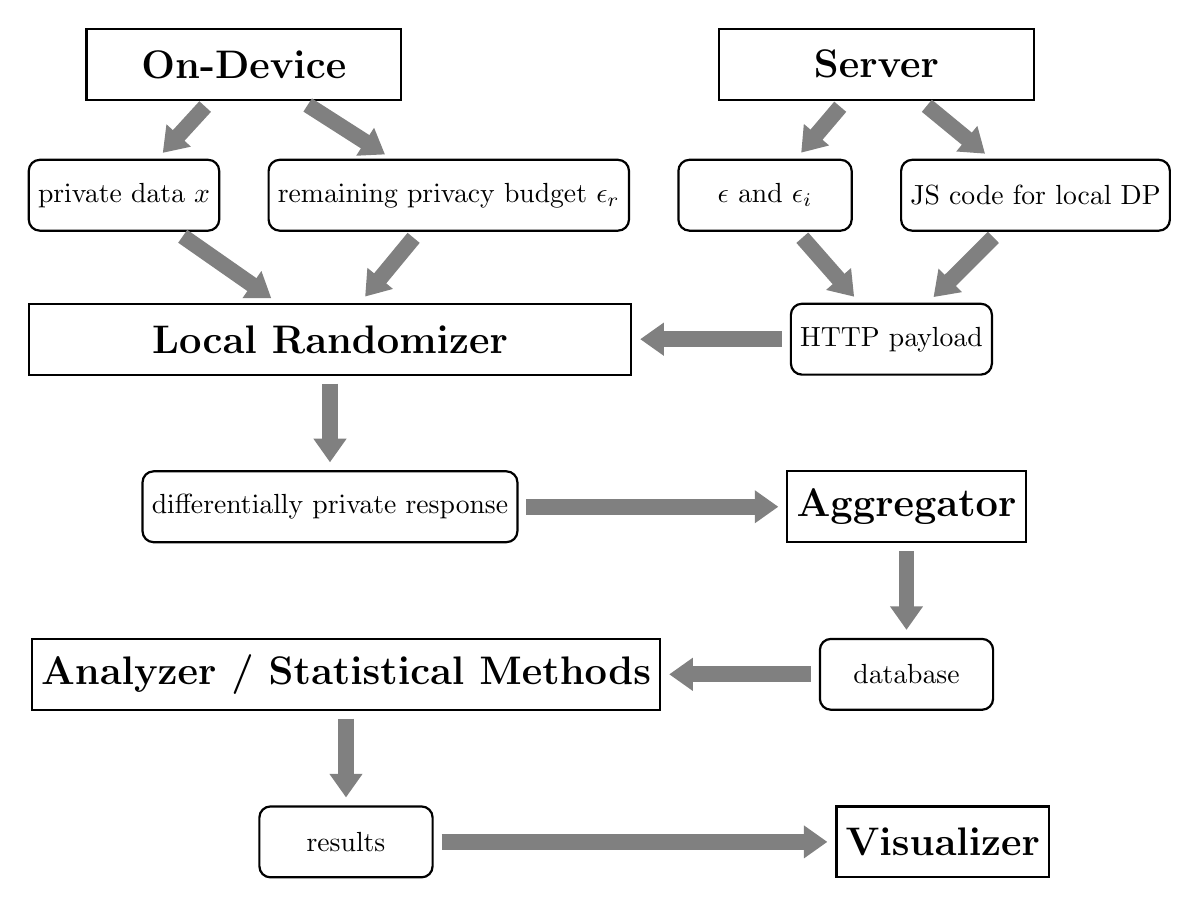
\begin{tikzpicture}[
node distance= 12mm and 6 mm,
inout/.style = {minimum width=#1,
                draw, thick, rounded corners, 
                minimum height=9mm, align=center},
inter/.style = {minimum width=#1,
                draw, thick, minimum height=9mm,
                font=\Large\bfseries},
Arrow/.style = {line width=2mm, draw=gray, 
                -{Triangle[length=3mm,width=4mm]},
                shorten >=1mm, shorten <=1mm},
                    ]
\node[inout=22mm]               (a)   {private data $x$};
\node[inout=22mm,right=of a]    (b)   {remaining privacy budget $\epsilon_r$};
\node[inout=22mm,right=of b]    (c)   {$\epsilon$ and $\epsilon_i$};
\node[inout=22mm,right=of c]    (d)   {JS code for local DP};
\path (a) -- (b) coordinate[midway] (a_b_mid);
\path (c) -- (d) coordinate[midway] (c_d_mid);

\path   let \p1 = (a.west),
            \p2 = (b.east),
            \n1 = {veclen(\x2-\x1,\y2-\y1)} in 
        node[inter=\n1, minimum width=4cm, above=of a_b_mid] (o) {On-Device}
        node[inter=\n1,
             below right=9mm and 0mm of a.south west] (f) {Local Randomizer};
                                        
\path   let \p1 = (c.west),
            \p2 = (d.east),
            \n1 = {veclen(\x2-\x1,\y2-\y1)} in 
        node[inter=\n1, minimum width=4cm, above=of c_d_mid] (s) {Server}
        node[inout=22mm,
             below=of c_d_mid, right=2 cm of f] (g) {HTTP payload};
             
\node[inout=22mm,below=of f]    (h)   {differentially private response};
\node[inter=22mm,right=3.4 cm of h]    (i)   {Aggregator};

\node[inout=22mm,below=of i]    (j)   {database};
\node[inter=22mm,left=2 cm of j]    (k)   {Analyzer / Statistical Methods};

\node[inout=22mm,below=of k]    (l)   {results};
\node[inter=22mm,right=5.1 cm of l]    (m)   {Visualizer};

\draw[Arrow]    (o) -- (a);
\draw[Arrow]    (o) -- (b);
\draw[Arrow]    (s) -- (c);
\draw[Arrow]    (s) -- (d);
\draw[Arrow]    (a) -- (f);
\draw[Arrow]    (b) -- (f);
\draw[Arrow]    (c) -- (g);
\draw[Arrow]    (d) -- (g);
\draw[Arrow]    (g) -- (f);
\draw[Arrow]    (f) -- (h);
\draw[Arrow]    (h) -- (i);
\draw[Arrow]    (i) -- (j);
\draw[Arrow]    (j) -- (k);
\draw[Arrow]    (k) -- (l);
\draw[Arrow]    (l) -- (m);
\end{tikzpicture}

\bigskip

\subsection{Server}

\noindent

Our local differential privacy framework starts at the server, where each experiment is created and its parameters initialized. When an experiment is created, it is given a total privacy budget $\epsilon$ as well as a per release privacy budget $\epsilon_i$.

\bigskip

Additionally, the data analyst will have be able to choose what type of experiment he or she desires, whether it be randomized response, a Hadamard Count Mean Sketch, or some other differentially private method of collecting data. This is where the modularity of our framework comes in -- if the desired data collection method is not already available within our framework, the analyst will be able to craft their own method and substitute it in. In the same vein, the analyst will be able to choose their desired composition theorem, whether it be basic, our advanced composition theorem, or some other composition theorem proposed in the future by another researcher.

\bigskip

Once these parameters are chosen, the server will craft JavaScript code corresponding to this differentially private mechanism, put it in an HTTP payload along with the $\epsilon$ and $\epsilon_i$ parameters, and send it to the device. Crucially, once the total privacy budget $\epsilon$ is chosen, it cannot be increased or reset, thus preventing the analyst from violating the privacy budget or misleading users.

\subsection{Local Randomizer}

\noindent

The local randomizer performs the crucial differential privacy steps in our framework. All interactions with the user's private data $x$ are performed on-device, and are not uploaded to the cloud. Crucially, the entire code for the randomizer is written in a single JavaScript file, and is easily auditable by third parties.

\bigskip

Once the randomizer is downloaded to the device, it starts by initializing the total privacy budget and storing it locally on-device. Once this budget is stored on-device in JavaScript's ``local storage,'' it cannot be cleared or augmented from the server without changes to the JavaScript code itself, which would be caught by third party auditors. However, our framework does allow for the server to change the per-response privacy budget $\epsilon_i$, in the event that it is discovered that more or less utility per-query is required. However, this functionality is dependent on the composition theorem used (advanced composition would require additional calculations to ensure that privacy is not lost).

\bigskip

After the randomizer is downloaded and the privacy budget initialized, the JavaScript code is ready to accept the private data from the user. This function can be called directly by the user's device in the background, or can be attached to a web interface to be presented to the user if the desired data is survey-based rather than usage-based. Crucially, since the entire process involves only JavaScript code (and some HTML/CSS, if desired), this framework is cross-platform and will work on virtually every modern device, no matter whether it is a supercomputer or a lightweight IoT sensor.

\bigskip

The function, when called, takes the user's private data $x$ and first determines if there is enough privacy budget $\epsilon_r$ remaining to perform the analysis. If not, it will refuse to submit the user's data and exit out. If there is enough privacy budget, it will subtract the correct amount and update the privacy budget $\epsilon_r$ (based on the composition theorem being used), perform the differentially private release (whether it be randomized response or some other method), and upload the results to the server.

\subsection{Aggregator}

\noindent

Now back on the server, our framework will collect each response and aggregate them, keeping track of which experiment each data sample is for. When storing the data, it will only keep the user's response and nothing else. For demonstration purposes, we keep a random ID string associated with each response so each participant can recognize their data in the results, and while it does not compromise privacy it is also not strictly necessary.

\subsection{Analyzer / Statistical Methods}

\noindent

Once all the data has been aggregated, it is passed to an analyzer that can perform different statistical methods on the data. For a simple randomized response, for example, it could simply calculate the estimated population mean with the correct scaling factor. For something more complicated like a Hadamard Count Mean Sketch, it could perform the necessary dictionary sampling to calculate the true counts of each phrase. The aggregator is also extensible to inference tools like differentially private stochastic gradient descent, which would allow us to train a model on the data. Since all the data is aggregated at a different stage in the pipeline, the modular nature of our framework allows us to switch up the analysis tools without having to re-write our pipeline from scratch.

\subsection{Visualizer}

\noindent

Once our data is analyzed and turned into actionable results, these results are passed into a visualizer that helps us understand what the data means. This could be as simple as a confidence interval graph for our population mean, or as complicated as a model of a gradient surface.

\section{Demo}

\subsection{Setup}

\noindent

For demonstration purposes, we chose to implement a simple randomized response mechanism accessible via a barebones Flask website. The code for this demonstration is available on \href{https://github.com/andrew-shackelford/CS-208-Final-Project/tree/master/Website}{GitHub}. To run it locally on your machine, simply \cl{cd} into the \cl{Website} directory, set the environment by running \cl{export FLASK_APP=application.py}, and execute \cl{flask run}.

\bigskip

Alternatively, we have also hosted the website publicly using PythonAnywhere, and it will be available for the near future at \href{http://cs208.pythonanywhere.com}{http://cs208.pythonanywhere.com}.

\subsection{Usage}

\noindent

Our website has two main user-facing functions, as well as a debug function for demonstration purposes.

\subsubsection{Submitting Data}

\noindent

As a single user, you can submit your data to the experiment by clicking on the ``Submit Data'' option in the navbar, choosing the experiment you wish to submit data to, and then clicking the ``True'' or ``False'' option. The submit page also displays the total privacy budget, the privacy budget per response, as well as the user's privacy budget remaining. Upon attempting to submit data, the page will redirect to either a success or failure page, depending on whether there was enough privacy budget left.

\subsubsection{Submitting Multiple Data}

\noindent

For demonstration purposes, we have added functionality to allow the submission of multiple data each with a certain probability of being True/False, as a tool to show how the calculated population mean will converge on the actual population mean as the number of responses increases. To use this function, click on the ``Submit Multiple Data'' option in the navbar, choose your dataset, desired population mean (on a $[0, 1]$ scale) and number of responses, and then click ``Perform Randomized Response''. Since this functionality is really only for debug purposes and was tacked on at the end of our project, each submission sends an individual POST request, which can take a good deal of time for large numbers of responses. As a result, we display an alert when the responses finish submitting. Additionally, we hard-coded the $\epsilon_i$ value to $1$ simply because it made adding this functionality to our website easier -- in the future we would improve this, or realistically remove the functionality altogether since it is only for demonstration purposes. 

\subsubsection{Viewing Data}

\noindent

To view the data, click on the ``View Data'' option in the navbar. Then, after choosing the dataset you'd like to view data from, the website will display the calculated population mean, as well as each individual response's ID and value. This allows each person to see that their response was indeed collected for demonstration purposes.

\section{Future Steps}

\noindent

In the future, we'd like to expand our framework by adding more data gathering, analyzing, and visualization methods. There are many different types of data collected using local differential privacy, and we'd like to support them all. Additionally, our current demo framework is not as modular as we'd like it to be. In the future, we'd like to re-write it to be truly modular and open-source it with appropriate documentation, so that any data analyst can add their own features in an easy and extensible manner.

\newpage

\phantomsection
\addcontentsline{toc}{section}{References}

\begin{thebibliography}{9}
\bibitem{apple} 
\textit{Learning with Privacy at Scale}. Apple Machine Learning Journal, December 2018. \\ \texttt{https://machinelearning.apple.com/2017/12/06/learning-with-privacy-at-scale.html}
 
\bibitem{tang_et_al} 
Jun Tang, Aleksandra Korolova, Xiaolong Bai, Xueqiang Wang, and Xiaofeng Wang. \textit{Privacy Loss in Apple's Implementation of Differential Privacy on MacOS 10.12}. arXiv, September 8, 2017. \\
\texttt{https://arxiv.org/abs/1709.02753}

\bibitem{google}
\'{U}lfar Erlingsson, Vasyl Pihur, and Aleksandra Korolova. \textit{RAPPOR: Randomized Aggregatable Privacy-Preserving Ordinal Response}. Google Research, November 2014. \\
\texttt{https://research.google.com/pubs/archive/42852.pdf}
 
\bibitem{microsoft} 
Bolin Ding, Jana Kulkarni, and Sergey Yekhanin. \textit{Collecting Telemetry Data Privately}. Microsoft Research, December 8, 2017. \\
\texttt{https://www.microsoft.com/en-us/research/blog/collecting-telemetry-data-privately/}

\bibitem{ektelo}
Dan Zhang, Ryan McKenna, Ios Kotsogiannis, Michael Hay, Ashwin Machanavajjhala, and Gerome Miklau. \textit{EKTELO: A Framework for Defining Differentially-Private Computations}. SIGMOD, June 2018. \\
\texttt{https://dl.acm.org/citation.cfm?id=3196921}

\bibitem{psi}
Marco Gaboardi, James Honaker, Gary King, Jack Murtagh, Kobbi Nissim, Jonathan Ullman, and Salil Vadhan. \textit{PSI ($\mathit{\Psi}$): a Private Data Sharing Interface}. Privacy Tools Project, August 7, 2018. \\
\texttt{https://arxiv.org/abs/1609.04340}

\bibitem{pinq}
Frank McSherry. \textit{Privacy Integrated Queries:
An Extensible Platform for Privacy-Preserving Data Analysis}. Microsoft Research, September 2010. \\
\texttt{https://www.microsoft.com/en-us/research/publication/privacy-integrated-queries-2/}

\bibitem{dwork}
Cynthia Dwork, Frank McSherry, Kobbi Nissim, and Adam Smith. \textit{Calibrating Noise to Sensitivity in Private Data Analysis}. TCC, March 2006. \\
\texttt{https://dl.acm.org/citation.cfm?id=2180305}

\end{thebibliography}

\newpage

\begin{appendices}

\section{\cl{advanced_composition.py}}
\label{appendix:advanced_composition}
\begin{lstlisting}
"""
Andrew Shackelford
ashackelford@college.harvard.edu

Peter Chang
chang04@college.harvard.edu

CS 208 - Spring 2019
Final Project: A Modular System for Local Differential Privacy
"""

import numpy as np
import matplotlib.pyplot as plt
from scipy.stats import binom

# calculate randomized response probability for given epsilon
def rr_prob(epsilon):
    return np.exp(epsilon) / (1. + np.exp(epsilon))

# return basic composition theorem
def basic_composition(epsilon, n):
    return float(epsilon) / float(n)

# return our advanced composition theorem
def advanced_composition(epsilon, n):
    epsilon, n = float(epsilon), float(n)
    old_epsilon_i = 0.
    epsilon_i = epsilon / n
    eta = epsilon
    t = 0.001
    s = 1.

    # iterate until we reach our desired threshold of 0.001
    while True:
        a = binom.cdf(np.ceil(n / 2.) - 1, n, rr_prob(epsilon_i))
        b = 1. - rr_prob(epsilon)
        t = 0.001
        if np.abs(epsilon_i - old_epsilon_i) < t and np.sign(a - b) == 1:
            return epsilon_i
        if np.sign(a - b) != s:
            s = -s
            eta = eta / 2.
        old_epsilon_i = epsilon_i
        epsilon_i = epsilon_i + s * eta

# calculate results for different values of epsilon
def calculate_results():
    basic_results = {}
    advanced_results = {}
    for epsilon in [1, 2, 5, 10]:
        basic_x, basic_y = [], []
        advanced_x, advanced_y = [], []
        for n in range(1, 101):
            basic_x.append(n)
            basic_y.append(basic_composition(epsilon, n))
            advanced_x.append(n)
            advanced_y.append(advanced_composition(epsilon, n))

        basic_results[epsilon] = (basic_x, basic_y)
        advanced_results[epsilon] = (advanced_x, advanced_y)

    return basic_results, advanced_results

# graph results for different values of epsilon
def graph_results(basic_results, advanced_results):
    for idx, epsilon in enumerate(sorted(basic_results.keys())):
        plt.plot(basic_results[epsilon][0], basic_results[epsilon][1], label='basic')
        plt.plot(advanced_results[epsilon][0], advanced_results[epsilon][1], label='advanced')
        plt.legend(loc='upper right')
        plt.xlabel(r'$n$')
        plt.ylabel(r'$\epsilon_i$')
        plt.title(r'Composition for $\epsilon$ = ' + str(epsilon))
        plt.savefig('advanced_composition_'+ str(epsilon) + '.png', bbox_inches='tight')
        plt.clf()

def main():
    basic_results, advanced_results = calculate_results()
    graph_results(basic_results, advanced_results)

if __name__ == "__main__":
    main()
\end{lstlisting}


\end{appendices}

\end{document}